% !TeX root = ../main.tex

\appendix{B}{風力機組規格}

本文研究的案例分析中,採用\uline{澎湖}地區作為示範,根據表 \ref{table: Taiwan Wind Farm Data} 的我國風力發電場址資料所示,該地區設有 Enercon E40/600 Model 與 Enercon E44/900 Model 風力機組,下述為此二風力機組之規格資料。

\section{Enercon E40/600 Model}

\subsection*{風機規格資料}

\begin{itemize}
  \item 額定功率 (Rated Power) :$600$ \si{\kW}
  \item 轉子直徑 (Rotor Diameter) :$40$ \si{\meter}
  \item 掃掠面積 (Swept Area) :$1,257$ \si{\meter\squared}
  \item 能量密度 (Power Density) :$2.1$ \si{\meter\squared}/\si{\kW}
  \item 葉片數量 (Number of Blades) :$3$ 片
  \item 葉輪最小額定轉速 (Minimum Rotor Speed) :$18$ \si{rd}/\si{\min}
  \item 葉輪最大額定轉速 (Maximum Rotor Speed) :$34.5$ \si{rd}/\si{\min}
  \item 額定風速 (Rated Wind Speed) :$13$ \si{m}/\si{s}
  \item 切入風速 (Cut-in Wind Speed) :$2.5$ \si{m}/\si{s}
  \item 切出風速 (Cut-off Wind Speed) :$25$ \si{m}/\si{s}
\end{itemize}

\subsection*{風機功率曲線}

\begin{figure}[htbp]
  \centering
  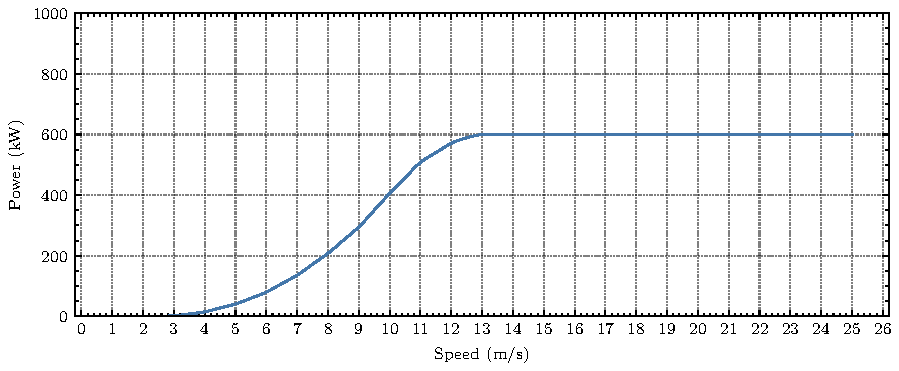
\includegraphics[width=\textwidth]{Enercon E40 600 Model}
  \caption{Enercon E40/600 Model 風機功率曲線}
  \label{figure: Enercon E40/600 Model}
\end{figure}

\section{Enercon E44/900 Model}

\subsection*{風機規格資料}

\begin{itemize}
  \item 額定功率 (Rated Power) :$900$ \si{\kW}
  \item 轉子直徑 (Rotor Diameter) :$44$ \si{\meter}
  \item 掃掠面積 (Swept Area) :$1521$ \si{\meter\squared}
  \item 葉片數量 (Number of Blades) :$3$ 片
  \item 葉輪最小額定轉速 (Minimum Rotor Speed) :$16$ \si{rd}/\si{\min}
  \item 葉輪最大額定轉速 (Maximum Rotor Speed) :$34.5$ \si{rd}/\si{\min}
  \item 額定風速 (Rated Wind Speed) :$17$ \si{m}/\si{s}
  \item 切入風速 (Cut-in Wind Speed) :$3$ \si{m}/\si{s}
  \item 切出風速 (Cut-off Wind Speed) :$25$ \si{m}/\si{s}
\end{itemize}

\subsection*{風機功率曲線}

\begin{figure}[htbp]
  \centering
  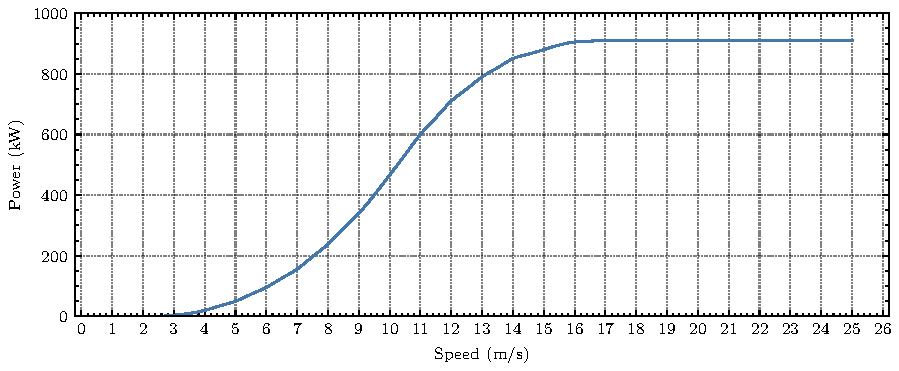
\includegraphics[width=\textwidth]{Enercon E44 900 Model}
  \caption{Enercon E44/900 Model 風機功率曲線}
  \label{figure: Enercon E44/900 Model}
\end{figure}
